\documentclass[../main]{subfiles}
\ifSubfilesClassLoaded{
    \addbibresource{../Biblio/biblio.bib}
    \dominitoc
    \tableofcontentsfile
    \pagenumbering{arabic}
    \setcounter{page}{1}
    \setcounter{chapter}{4}
}{}
\begin{document}
\chapter{Indicateurs statistiques de l'apprentissage des données multimodales\label{chap:indicateur}}
\graphicspath{{05-Indicateur/figures},{./figures/}}
\minitoc

Dans le chapitre \ref{chap:repr}, nous avons présenté différents tracés permettant d'évaluer comment l'architecture de cartes extrait une représentation interne du modèle d'entrée lors de l'apprentissage sur des cartes et données en une dimension.
Nous avons observé que l'apprentissage du modèle se caractérise notamment par le fait que chaque carte dissocie les BMUs en fonction du modèle d'entrées global et non seulement de son entrée externe. 
La variable cachée $U$, représentant le modèle d'entrées, est alors une fonction du BMU $\bmu$ dans chacune des cartes de l'architecture, comme rappelé sur la figure~\ref{fig:upi_chap4}.
Nous souhaitons définir un indicateur numérique caractérisant cette propriété, c'est-à-dire caractérisant que $U$ est fonction de $\bmu$ dans chaque carte. Cet indicateur nous permettra  de comparer plusieurs expériences entre elles de façon numérique.
Les tracés sont réalisables pour une variable cachée $U$ en en une dimension~; un indicateur numérique nous permettra aussi d'évaluer l'apprentissage lorsque la dimension de $U$ est plus grande.

Nous avons défini les expériences en termes de variables aléatoires. La théorie de l'information de Shannon \cite{Shannon1948AMT} apporte un modèle mathématique qui permet de manipuler et encoder ces variables et quantifier l'information partagée entre leurs distributions.
Nous proposerons dans ce chapitre des indicateurs permettant d'évaluer l'apprentissage du modèle par l'architecture de cartes. 

\begin{figure}
    \centering
    \includegraphics[width=0.7\textwidth]{xu_yu_both_chap4.pdf}
    \caption{Rappel~: comparaison de $U$ en fonction de $\bmu\m{1}$ dans l'expérience exemple à deux cartes, sur des entrées sous forme de cercle. Ce nuage de point fait apparaître une relation semblant bijective entre $U$ et $\bmu\m{1}$. Nous définiront un indicateur permettant de représenter numériquement cette propriété.
    \label{fig:upi_chap4}}
\end{figure}

\subsection*{Indicateurs envisagés}

Plusieurs méthodes permettent d'évaluer une relation statistique existant entre deux signaux.
Parmi ceux-ci, citons le coefficient de corrélation (Pearsons' R) et le ratio de corrélation, illustrés en figure~\ref{fig:signaux}, ainsi que l'information mutuelle.
Le coefficient de corrélation, connu également comme le coefficient de Pearson, est une mesure statistique mesurant une dépendance linéaire entre des échantillons $X$ et $Y$. Il est défini par le rapport de la covariance des variables et le produit de leurs écarts-type:
\begin{equation}
    r = \frac{Cov(X,Y)}{\sigma_X \sigma_Y} 
\end{equation}
Ce coefficient est symétrique, vaut 0 si les variables sont indépendantes et 1 s'il existe une relation linéaire entre $X$ et $Y$. Il mesure spécifiquement une relation linéaire entre les variables. 
D'un point de vue apprentissage, $r$ mesure la qualité de l'approximation des valeurs de $Y$ par une fonction linéaire sur $X$. 
Sur la figure~\ref{fig:signaux}, les valeurs obtenues par une régression linéaire aux moindres carrés sont indiquées en rouge. Le coefficient $r$ mesure comment ces valeurs approximent $Y$. 

Le ratio de corrélation $\eta(Y;X)$ est une autre mesure statistique entre des données $X$ et $Y$. Ce coefficient n'est pas symétrique. Il mesure à quel point les valeurs de $Y$ sont approximées par une fonction de $X$ et permet donc de mesure une dépendance fonctionnelle non linéaire entre deux échantillons.
Il est défini par~:
\begin{equation}
    \eta(Y;X) = 1 - \frac{\mathbb{E}(Var(Y|X)))}{Var(Y)}
\end{equation}

Nous détaillerons le calcul de ce coefficient dans la suite de ce chapitre. Notons seulement que la fonction $\varphi(x) = \mathbb{E}(Y|X = x)$, utilisée pour le calcul de $Var(Y|X)$, est la fonction approximant le mieux les valeurs des paires $(X,Y)$ au sens des moindres carrés. Cette fonction est tracée en rouge sur la figure~\ref{fig:signaux}
Le ratio de corrélation mesure alors la qualité de cette approximation. Il vaut 1 si $Y$ est une fonction de $X$ et 0 si les variables sont complètement indépendantes. 

Enfin, l'information mutuelle, contrairement aux mesures présentées ci-dessus, est une grandeur probabiliste.
Elle évalue une relation quelconque et non seulement fonctionnelle entre les distributions des variables $X$ et $Y$. Elle vaut 0 si et seulement si les variables sont indépendantes et est maximale lorsque qu'il existe une bijection entre les deux variables aléatoires.
Son application à des échantillons statistiques passe par l'estimation des distributions des variables ou de leur entropie.

Nous avons remarqué dans les cas d'exemples présentés au chapitre précédent que l'apprentissage du modèle se traduit par une relation fonctionnelle entre les valeurs de $U$ et la position du BMU $\Pi$ dans chaque carte. 
Nous cherchons dans ce chapitre à définir des indicateurs de l'apprentissage du modèle par les cartes. Le ratio de corrélation, qui permet de mesurer une relation fonctionnelle quelconque entre deux variables apparaît comme un indicateur pertinent de cet apprentissage.

D'autre part, l'information mutuelle mesure également l'existence d'une relation fonctionnelle entre deux variables aléatoire, étant donné qu'elle vaut 1 lorsqu'il existe une bijection entre $X$ et $Y$.
L'hypothèse que l'apprentissage du modèle se traduit dans chaque carte par le fait que $U$ est une fonction du BMU dans chaque carte reste à vérifier, en particulier en dimension supérieure à 1.Nous avons par ailleurs noté qu'il n'est pas souhaitable que $U$ soit fonction de la position du BMU dans toutes les cartes d'une architecture, mais plutôt que la représentation de $U$ soit distribuée entre les cartes, tout en présentant de la redondance en terme d'information.
Le calcul de l'information mutuelle entre les éléments de réponse d'une carte et ses entrées sera ainsi pertinent à explorer pour compléter la compréhension du modèle. 
L'information mutuelle est par ailleurs largement utilisée comme métrique, indicateur ou fonction de coût dans de nombreux domaines, donc un grand nombre de méthodes d'estimation et d'implémentation existent pour son calcul sur des données statistiques.
L'information mutuelle n'est pas normalisée, mais il en existe des variantes normalisées que nous présenterons et utiliserons dans ce chapitre. 

\begin{figure}
    \includegraphics[width=\textwidth]{mi_cr.pdf}
    \caption{Le coefficient de corrélation de Pearsons $r$, en figure de gauche, mesure une relation linéaire entre les variables X et Y. Le ratio de corrélation, au centre, cherche à déterminer l'existence d'une fonction entre Y et X. \label{fig:signaux}}
\end{figure}

% \begin{itemize}
%     \item Avantages du correlation ratio: mesure précisément une relation fonctionnelle quelconque, est à valeur dans 0,1. Désavantages: besoin de passer par l'estimation des densités de proba, en particulier $U|\bmu$, donc peu pratique quand la dimension augmente.
%     \item Information mutuelle : mesure une relation statistique quelconque. Largement utilisé, donc de nombreuses méthodes fiables d'estimation existent, y compris pour des dimensions supérieures. Normalisation possible pour définir un indicateur compris entre 0 et 1. Est maximale lorsque qu'il existe une bijection entre les deux variables, ce qui est ce qu'on veut mesurer.
% \end{itemize}

Nous présenterons dans ce chapitre d'abord un indicateur s'appuyant sur le ratio de corrélation, qui répond spécifiquement à nos besoins lorsque les cartes sont en une dimension. 
Nous explorons ensuite un indicateur s'appuyant sur l'information mutuelle.
Cet indicateur permet de mesurer une dépendance fonctionnelle entre les deux variables mais dépend beaucoup de la méthode d'estimation utilisée et est limité si $U$ est de grande dimension. Enfin, nous discuterons des possibilités d'utilisation de l'information mutuelle comme indicateur d'apprentissage dans une structure de cartes.

\section{Utilisation du ratio de corrélation comme mode d'évaluation}

Nous avons observé sur les différences expériences présentées en une dimension que l'apprentissage du modèle se traduit par l'existence d'une dépendance fonctionnelle entre $U$ et le BMU $\bmu\m{i}$ de chaque carte.
Le ratio de corrélation $\eta(\bmu\m{i},U)$ permet de mesurer un coefficient de dépendance non-linéaire entre deux variables, ce qui correspond à une relation fonctionnelle. Il atteint la valeur de 1 lorsque $U$ est fonction de la première variable $\bmu\m{i}$ et est nul lorsque les deux variables sont statistiquement indépendantes. Nous pouvons donc utiliser cet indicateur pour vérifier cette propriété.

\subsection{Définition}

La mesure de la dépendance fonctionnelle entre deux variables $X$ et $Y$ peut se décomposer en deux étapes~:
\begin{enumerate}
    \item Trouver une fonction $\varphi(X)$ qui approxime les valeurs de $Y$
    \item Mesurer la qualité de l'approximation.
\end{enumerate}

En considérant deux variables $x \in \Omega_X$, $y \in \Omega_Y$, la fonction approchant le mieux l'ensemble de variables $(x,y)$ au sens des moindres carrés est la fonction~:
\begin{equation}
    \varphi(x) = \mathbb{E}(Y|X = x), x \in \Omega_X
\end{equation}

Un exemple d'estimation de $\varphi(x)$ est illustré en figure~\ref{fig:cr_box}, estimée par discrétisation des valeurs de $X$. $\varphi(x)$ est une variable aléatoire à valeurs dans $\Omega_X$.

Le ratio de corrélation $\eta$ se définit à partir de $\varphi$ et mesure la qualité de l'approximation des valeurs de $Y$ par la fonction $\varphi$ au sens des moindres carrés en calculant la moyenne des variances de la variable $Y|X$ pour chaque valeur possible de $X$. 

\begin{equation}\label{eq:cr}
   \eta(Y;X) = 1 - \frac{\mathbb{E}(Var(Y|X))}{Var(Y)}
\end{equation}

$\mathbb{E}(Var(Y|X))$ représente la moyenne des écarts de $Y|X=x_i$ à sa valeur moyenne en $x_i$ $\mathbb{E}(Y|X=x_i)$ pour une valeur de $X = x_i$ donnée. 
En effet, en notant $Z$ la variable aléatoire $Y | X=x_i$~: 
$$ Var(Y|X=x_i) = \mathbb{E}((Z - \mathbb{E}(Z))^2)$$
$$ Var(Y|X=x_i) = \mathbb{E}((Z - \varphi(x_i))^2)$$

Lorsque la dépendance entre $Y$ et $X$ est fonctionnelle, les valeurs de $Y|X = x_i$ sont très proches de $\varphi(x_i)$  pour toutes les valeur de $x_i$ et $\mathbb{E}(Var(Y|X=x_i))$ est faible partout. La variance est nulle lorsqu'une valeur de $X$ correspond à un seul point pour $Y$, c'est-à-dire une relation fonctionnelle. 
Inversement, quand $Y$ et $X$ sont indépendantes, $Var(Y|X=x_i) = Var(Y)$ pour tout $x_i$, donc $\mathbb{E}(Var(Y|X)) = Var(Y)$ et $\eta(Y;X) = 0$.

La définition du coefficient se retrouve plus généralement sous une forme modifiée de l'équation~\ref{eq:cr}~:
par la définition des variances conditionnelles,
$$Var(Y) = \mathbb{E}(Var(Y|X)) + Var(\mathbb{E}(Y|X))$$
Soit~:
\begin{equation}
    \eta(Y;X) = \frac{Var(\mathbb{E}(Y|X))}{Var(Y)}
\end{equation}

Le ratio de corrélation n'est pas symétrique. 
Par le fait qu'il s'appuie sur un rapport, il n'est pas sensible à une transformation linéaire de $Y$ et est sans unité.

\begin{figure}
    \centering
    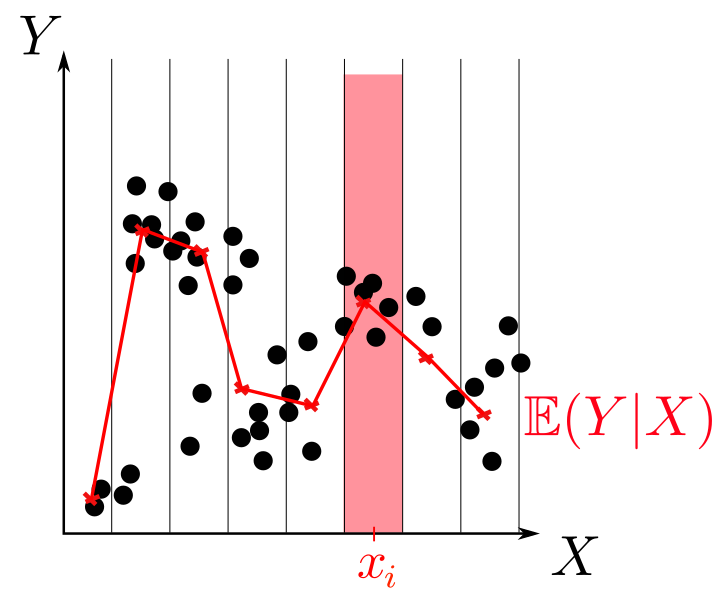
\includegraphics[width=0.6\textwidth]{boxes_CR.pdf}
    \caption{Exemple d'approximation non-linéaire de la relation entre $X$ et $Y$ par $\mathbb{E}(Y|X)$. Cette approximation est ici réalisée en discrétisant les valeurs de $X$. La valeur de la fonction pour chaque $x_i$ est alors la moyenne des valeurs de $Y$ sur l'intervalle considéré.\label{fig:cr_box}}
\end{figure}

\subsection{\'Evolution du ratio de corrélation au cours de l'apprentissage des cartes CxSOM}

Nous pouvons utiliser le ratio de corrélation pour mesurer la dépendance fonctionnelle existant dans chaque carte entre les valeurs de $U$ et l'ensemble des BMU d'une carte $\bmu\m{i}$, sur les différentes ensembles d'entrées étudiés au chapitre précédent.
Les valeurs $\bmu\m{1}$ et $\bmu\m{2}$ étant des valeurs discrètes, $\mathbb{E}(U|\bmu\m{i})$ est estimée par la moyenne des valeurs de $U$ ayant pour BMU la même valeur $\bmu\m{i}$. 
En figure~\ref{fig:cr_xp}, nous traçons les distributions de $U$ en fonction de $\bmu\m{1}$ et $\bmu\m{2}$, dans le cas de l'architecture CxSOM et des cartes indépendantes, pour des entrées placées sur le cercle 2D. Nous y représentons la fonction $\mathbb{E}(U|\bmu\m{i})$ en rouge.
Le ratio de corrélation apparaît ici comme une bonne mesure de la relation fonctionnelle existant entre $U$ et $\bmu$. Le ratio de corrélation est très proche de 1 dans chaque carte de CxSOM, traduisant le fait que $U$ est une fonction du BMU dans chaque carte.

La figure~\ref{fig:cr_bruit} présente les mêmes paramètres tracés dans le cas ou l'expérience est réalisée sur des données bruitées, en l'occurence un anneau. $U$ n'est alors plus vraiment une fonction du BMU, mais en reste proche. 
Le ratio de corrélation traduit correctement cette proximité et est plus élevé dans chaque carte de l'architecture que pour une carte seule.

\begin{table}
    \centering
    \caption{Comparaison des valeurs du ratio de corrélation sur plusieurs expériences.}
    \begin{tabular}{*7c}
        \toprule
        & \multicolumn{2}{c}{Entrées} & \multicolumn{2}{c}{CxSOM} & \multicolumn{2}{c}{Cartes Simples} \\
        \cmidrule(lr){2-7}
         & $\eta(U;\inpx\m{1})$ & $\eta(U;\inpx\m{2})$  & $\eta(U;\bmu\m{1})$ & $\eta(U;\bmu\m{2})$  & $\eta(U;\bmu\m{1})$ & $\eta(U;\bmu\m{2})$ \\    
        \midrule
        Cercle &   $0.45 $    & $0.84$  &  $0.98$ & $0.99$ & $0.49$ & $0.84$      \\
        Anneau &  $0.43$      &  $0.83$      & $0.97$ & $0.93$ & $0.44$ & $0.98$ \\
        Lissajous &  $0.81$     &  $0.80$ & $0.96$ & $0.94$  & & \\
        \bottomrule
    \end{tabular}
\end{table}
Enfin, nous traçons en figure~\ref{fig:cr_evol} l'évolution du ratio de corrélation sur les 200 premiers pas d'apprentissage de deux cartes sur un cercle, connectées et non connectées. Les mesures sont réalisées sur 10 expériences réalisées sur des distributions d'entrées identiques et moyennées.
Nous remarquons que $\eta$ reste inférieur dans le cas ou les cartes sont connectées que non connectées. 
Le ratio de corrélation traduit une relation fonctionnelle mais ne prend pas en compte l'aspect continu des positions. Ainsi, à partir du moment ou deux positions différentes sont BMU pour une même entrée, même lorsque les poids ne sont pas organisés, le ratio de corrélation est élevé. Le ratio de corrélation apparaît ainsi sur la figure prendre à une valeur élevée tout au long de l'apprentissage. Il ne traduit pas d'organisation des poids.
$\eta(U;\bmu\m{2})$ est bien plus élevé sur $\eta(U;\bmu\m{1})$, ce qui apparaît également sur les figures~\ref{fig:cr_xp} et \ref{fig:cr_bruit}, à cause de la relation entre entrées.
Intuitivement, on voudrait que les deux expériences aient un indicateur similaire.
Bien que les valeurs de $\eta$ soient normalisées, il est donc compliqué d'utiliser cette métrique comme valeur absolue pour comparer des expériences~; mais seulement la comparer à $\eta(U;\inpx\m{1})$ et $\eta(U;\inpx\m{2})$

\begin{figure}
    \centering\includegraphics[width=0.8\textwidth]{correlation_ratio_cercle0.pdf}
    \caption{Tracé du ratio de corrélation et de $\varphi$ sur des entrées placées sur un cercle. Comparaison entre CxSOM et une carte simple \label{fig:cr_xp}}
\end{figure}

\begin{figure}
   \centering \includegraphics[width=0.8\textwidth]{xu_yu_both_anneau.pdf}
    \caption{Tracé du ratio de corrélation sur cartes CxSOM et cartes simples pour des entrées placées sur un anneau.\label{fig:cr_bruit}}
\end{figure}

\begin{figure}
    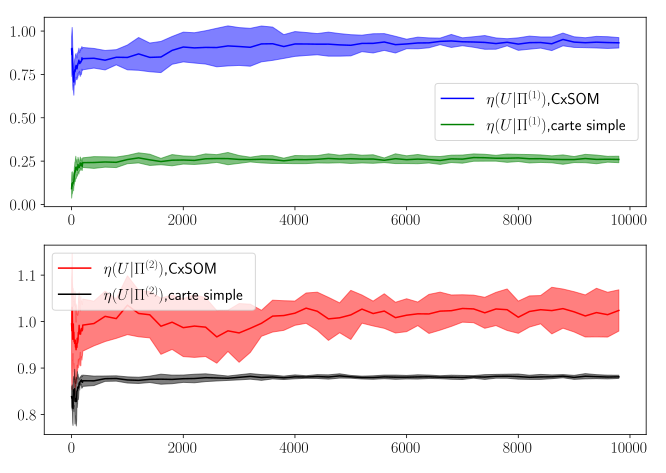
\includegraphics[width=\textwidth]{correlation_ratio_evolution_totale.pdf}
    \caption{\'Evolution du ratio de corrélation pendant l'apprentissage des cartes\label{fig:cr_evol}}
\end{figure}

\subsection{Discussion}

Le ratio de corrélation $\eta(U;\bmu)$ est une mesure statistique qui exprime par définition la relation fonctionnelle existant entre $U$ et $\bmu$, ce que nous cherchions à mesurer. Cette mesure nécessite de discrétiser les valeurs de $\Pi$ mais pas de $U$, ce qui est adapté aux cartes auto-organisatrices dans lesquelles $\Pi$ est en une ou deux dimensions. Il s'agit donc d'une bonne mesure de l'apprentissage de $U$ par une carte et est adaptable pour des cartes en 2D, ainsi que des $U$ en grande dimension.
Cependant, la valeur du ratio de corrélation dépend également de l'organisation originale des entrées.
L'utilisation du ratio de corrélation comme indicateur d'un bon apprentissage de $U$ par les BMUs n'est donc pertinent qu'en le comparant à sa valeur théorique $\eta(U;\bmu)$ ou à la valeur qu'il prend dans une carte auto-organisatrice indépendante.

\section{L'information mutuelle comme indicateur de l'apprentissage de $U$ par les BMUs}

Le ratio de corrélation est une bonne mesure de la relation fonctionnelle entre $U$ et $\bmu$ dans chaque carte. Cependant, nous ne voulons pas nous restreindre à la mesure de cette propriété comme indicateur de l'apprentissage du modèle par l'architecture~: un modèle pourrait être appris de façon distribuée dans une architecture comportant plus de cartes sans que $U$ soit une fonction du BMU.
Nous nous intéressons donc aux mesures d'information entre les éléments des cartes pris comme des variables aléatoires.

\subsection{Rappel des éléments de théorie de l'information}

Les notions d'\emph{entropie} et les valeurs associées, telle que l'\emph{information mutuelle} entre des variables aléatoires, sont des notions fondamentales de la théorie de l'information de Shannon. Ces quantités sont calculées à partir de la distribution des variables aléatoires.
L'entropie de Shannon d'une variable aléatoire $X$ à valeurs discrètes dans un ensemble $\Omega_X$, de distribution $P_X$, est notée $H(X)$ et définie par la formule : 
\begin{equation}
H(X) = - \sum_{x \in \Omega_X}{P_X(x)\textrm{log}(P_X(x))}
\end{equation}

L'entropie de Shannon concerne uniquement des variables discrètes.
Une autre version de l'entropie est définie pour des variables continues, l'entropie différentielle~:
\begin{equation}
    H(X) = - \int_{x \in \Omega_X}{p_X(x)\textrm{log}(p_X(x))dx}
\end{equation}
Avec $p_X$ la densité de probabilité de $X$.
    
Cette valeur n'est cependant pas la limite de l'entropie de Shannon calculée par discrétisation de $X$ en $N$ intervalles, $N \rightarrow \infty$.
L'entropie différentielle et l'entropie de Shannon sont donc deux quantités bien différentes.

L'entropie de Shannon se mesure en $bit/symbole$.
C'est une mesure de la quantité d'incertitude, ou de surprise, sur la valeur de la variable aléatoire $X$. Si la distribution de $X$ est concentrée autour d'un point, l'entropie est faible : lors d'une réalisation de $X$, l'observateur est \emph{plutôt certain} du résultat. En revanche, l'entropie est maximale lorsque $X$ suit une distribution de probabilité uniforme.
L'entropie s'interprète également comme la quantité moyenne d'information à fournir, en bits, pour coder une valeur de $X$.
De la même manière, on peut définir l'entropie conjointe de deux variables, qui est l'entropie de leur distribution jointe, et l'entropie conditionnelle, qui est l'entropie de leurs distributions conditionnelles.

Outre les entropies jointes et conditionnelles, l'existence d'une relation statistique entre deux variables aléatoires $X,Y$ à valeurs dans $\Omega_X,\Omega_Y$ se mesure par \emph{l'information mutuelle}.
Elle est définie par : 
\begin{equation}
 I(X,Y) = \sum_{x,y \in \Omega_X,\Omega_Y}{P_{XY}(x,y)\textrm{log}(\frac{P_{XY}(x,y)}{P_X(x)P_Y(y)})}
\end{equation}

Avec $P_XY$ la distribution de la variable aléatoire jointe $(X,Y)$
Cette valeur mesure la quantité d'information moyenne partagée entre les distributions $X$ et $Y$~: en moyenne, quelle information sur la valeur de $Y$ donne une valeur de $X$ et inversement, quelle information sur la valeur de $X$ donne une valeur de $Y$.

L'information mutuelle possède les propriétés suivantes~:
\begin{enumerate}
\item $I(X,Y) = 0 \Leftrightarrow \textrm{X et Y sont indépendantes}$. L'information mutuelle peut être vue une mesure de la distance entre la distribution jointe de $(X,Y)$, $P(X,Y)$ et la distribution correspondant à l'indépendance des variables, $P(X)P(Y)$.
\item\label{it:h} Elle s'exprime à partir de l'entropie de Shannon : $I(X,Y) = H(X) + H(Y) - H(X,Y) = H(X) - H(X|Y) = H(Y) - H(Y|X)$
\item Elle est symétrique : $I(X,Y) = I(Y,X)$
\item\label{it:eq} Pour toute fonction $f$, $I(X,Y) \geq I(X,f(Y))$. L'égalité est atteinte si et seulement si $f$ est \emph{bijective}.
\end{enumerate}

L'information mutuelle se calcule également à partir des densités de probabilité pour des variables à valeur continues de densités de probabilité $p_X$ et $p_Y$~:
\begin{equation}
    I(X,Y) = \int_{x \in \Omega_X}\in _ {y \in \Omega_Y }{p_{XY}(x,y)\textrm{log}(\frac{p_{XY}(x,y)}{p_X(x)p_Y(y)})dx \: dy}
\end{equation}

Contrairement à l'entropie, la valeur de l'information mutuelle pour des variables continues correspond bien à une limite des valeurs de l'information mutuelle discrète lorsque le nombre de catégories tend vers l'infini.
Cependant, dans le cas continu, les propriétés \ref{it:h} et \ref{it:eq} ne sont pas vérifiées. L'information mutuelle n'est en effet pas comparable à l'entropie différentielle.

Lors de l'analyse de CxSOM, on s'interroge plus généralement sur l'information que portent les positions des BMUs $\bmu$ d'une carte sur le modèle d'entrée.
Les éléments de la carte ont été définis en termes statistiques~; on peut donc utiliser l'information mutuelle comme une représentation de l'information partagée entre la position du BMU d'une carte et la variable paramétrant le modèle d'entrée, $U$.

\subsection{Méthodes d'estimation de l'information mutuelle}

L'information mutuelle et l'entropie sont des grandeurs définies à partir de la distribution des variables aléatoires. Ces distributions, dans notre cas, ne sont pas connues, nous devons donc estimer ces quantités à partir des échantillons de données.

La méthode classique d'estimation de l'information mutuelle et de l'entropie discrète est la méthode dite des \emph{histogrammes}.
Cette méthode s'appuie sur une estimation de la distribution des variables $U$,$\bmu$ et la distribution de la variable jointe $(U,\bmu)$ en discrétisant chacune des variables.
Cette méthode est représentée en figure~\ref{fig:binning}. Les variables $U$ et $\bmu$ sont discrétisées en \emph{boîtes} de centres $x_k$ et $y_k$ choisis.
Une distribution est alors estimée par: 
$$P(U = x_i) = \frac{n_{xi}}{N} $$ où $n_{xi}$ est le nombre d'échantillons de $U$ tombant dans la boîte de centre $x_i$ et $N$ le nombre de points. Le même procédé est réalisé pour $\bmu$ et $(U,\bmu)$. La précision de l'estimation peut être améliorée en choisissant des tailles de boîtes variables; nous utilisons ici la méthode simple avec des boites de taille fixe.
Pour des variables à valeur dans $[0,1]$, les centres sont définis par $x_k = \frac{k}{M}+\frac{1}{2M}$, avec $M$ le nombre de boîtes.
Cette discrétisation permet d'estimer les trois termes d'entropie $\hat{H}(\bmu,U)$, $\hat{H}(U)$ et $\hat{H}(\bmu)$ et d'en tirer l'information mutuelle~:
\begin{equation}
    \hat{I_x}(U,\bmu) = \hat{H}(U) + \hat{H}(\bmu) - \hat{H}(U,\bmu)
   \end{equation}

La valeur de cet indicateur dépend de la résolution choisie pour l'histogramme. L'estimateur  par histogramme converge vers la valeur théorique de l'information mutuelle continue lorsque la taille des boites tend vers 0, sous réserve que les densités de probabilité existent pour chaque variable.
Plus la taille des boîtes est petite, plus le nombre de points disponible pour l'estimation doit augmenter.
Notons que la méthode par histogrammes est limitée quand la dimension des entrées augmente.
Le nombre d'échantillons disponibles pour l'estimation doit augmenter exponentiellement avec la dimension des variables pour éviter le phénomène de "boîtes vides"~: à cause de la dispersion des données, de nombreuses boîte $(x_j,y_i)$ ne contiendront pas de points alors qu'elles auraient dû en contenir selon leur distribution; l'estimation de la distribution en ce point sera alors nulle, et l'estimation de l'indicateur faussée.


Une deuxième méthode souvent utilisée pour l'estimation de l'information mutuelle est l'estimateur par KNN (K-nearest neighbors) de Kraskov \cite{2004kraskov}.
Cet estimateur ne passe pas par l'estimation de la densité de probabilité, contrairement aux histogrammes, mais estime directement l'information mutuelle continue.
Le découpage de l'espace se fait en recherchant, pour un couple $(X,Y)$ les k plus proches voisins. Une information mutuelle locale est calculée dans cette zone de l'espace, suivant une formule permettant d'approximer les différences de logarithme par la fonction digamma $\psi$ : 
$$i_j(X,Y) = \psi(k) - \psi(n_{x_j} + 1) - \psi(n_{y_j} +1) + \psi(N)$$
Cette information mutuelle locale est ensuite moyennée sur l'ensemble des points: 
$$\hat{I}(X,Y) = \psi(k) - \langle\psi(n_{x_j} + 1) + \psi(n_{y_j} +1)\rangle + \psi(N)$$
L'estimateur de Kraskov est plus précis que l'estimateur par histogrammes et est moins sensible aux paramètres choisis pour son estimation qui sont le nombre de voisins considérés.

\begin{figure}
    \begin{minipage}{0.4\textwidth}
    \centering
    \includegraphics[width=\textwidth]{boxes}
    \caption{Méthode par histogrammes pour estimer les distributions des variables $U$ et $\bmu$. Les distributions sont estimées à partir de $n_{xj}$, $n_{yi}$ et $n_{zij}$, puis les valeurs de l'entropie $H$ et l'information mutuelle $I$ calculées.}
    \label{fig:binning}  
    \end{minipage}
    \hfill
    \begin{minipage}{0.4\textwidth}    
            \centering
            \includegraphics[width=0.8\textwidth]{kraskov.pdf}
            \caption{Découpage en KNN de Kraskov pour estimer l'entropie et l'information mutuelle des variables $X$ et $Y$. Les plus proches voisins du point rouge sont trouvés, en vert, et le processus est répété sur tous les points. Les valeurs de $n_x$ et $n_y$ permettent d'estimer directement l'entropie.}
            \label{fig:kraskov}
    \end{minipage}
    \end{figure}

\section{Définition d'un indicateur quantifiant la relation fonctionnelle entre $U$ et $\bmu$}

Dans un premier temps, nous avons cherché à définir un indicateur permettant de montrer que $U$ est une fonction du BMU à partir de l'information mutuelle, que nous avons utilisé en \cite{Gonnier2020ConsensusDS}. 
Nous décrivons ici une méthode que nous avons proposée avant de s'intéresser au ratio de corrélation. Ce dernier sera à privilégier par rapport à la méthode que nous décrivons ici pour montrer la relation fonctionnelle entre $U$ et $\bmu$. 

Nous définissons cet indicateur en normalisant l'information mutuelle $I(\bmu,U)$  par la valeur maximale qu'elle peut prendre dans une carte. Cette valeur maximale atteinte est $H(U)$, atteinte lorsque $U$ est une fonction de $\bmu$.
En effet, par construction, $\bmu$ est une fonction de $U$ dans une carte de Kohonen: l'algorithme est déterministe et une sortie est définie pour toute valeur de $U$. C'est-à-dire, $I(U,\bmu) = I (U, f(U))$.
Par propriété de l'information mutuelle, pour toute fonction $f$ et variables $X,Y$, $I(X,f(Y)) \leq I(X,Y) $. 
Donc, $I(U,\bmu) \leq I(U,U) = H(U)$
Cette valeur est atteinte si et seulement si $U$ et $\bmu$ sont en bijection, autrement dit, si et seulement si $U$ est aussi une fonction de $\bmu$.

Nous définissons donc l'indicateur $I_x$ de la relation fonctionnelle existant entre $U$ et $\bmu$ comme~:
\begin{equation}
I_x(U|\bmu) = \frac{I(\bmu,U)}{H(U)}
\end{equation}

Ce coefficient n'est pas symétrique et mesure l'information portée par le second terme sur le premier, relativement à la valeur maximale qu'il peut prendre ($H(U)$). On a $I_x(U|\bmu) \in [0,1]$. Cette valeur est une variante normalisée de l'information mutuelle est s'apparente au \emph{coefficient d'incertitude} entre $U$ et $\Pi$ et introduit en~\cite{Theil1961EconomicFA}.
$I_x$ vaut 1 lorsque $U$ est une fonction de $\bmu$, et $0$ lorsque les deux distributions sont indépendantes. Cette relation fonctionnelle entre $U$ et $\bmu$ est bien la propriété qu'on souhaite mesurer.

La normalisation de l'information mutuelle par l'entropie est uniquement valable dans le cas de variables aléatoires discrètes. Il est donc nécessaire dans ce cadre d'utilisation de considérer $\bmu$ et $U$ comme des variables discrètes et donc d'estimer l'information mutuelle et l'entropie par la méthode des histogrammes.


\subsection{Choix des paramètres d'estimation}

Pour mieux comprendre ce que représente l'information mutuelle discrète, comparons en figure~\ref{fig:exemple-limite} deux exemples de relations entre les variables $U$ et $\bmu$.
Dans le cas de gauche, la relation se rapproche d'une relation fonctionnelle, qu'on souhaite dans le cas de CxSOM, mais cette relation est bruitée. Dans le cas de droite, la relation n'est pas une fonction, mais elle est "précise": une valeur de $\bmu$ correspond à deux valeurs de $U$ et pas plus.

Dans le cas de gauche, l'estimation de l'information mutuelle continue par la méthode de Kraskov donne un coefficient d'incertitude assez faible. 
En effet, une valeur de $\bmu$ correspond à tout un intervalle de valeurs pour $U$. Sur le cas de droite, sa valeur est plus haute. En effet, une valeur de $\bmu$ correspond à deux valeurs de $U$, ce qui donne plus d'information que dans le premier cas de figure. Ce n'est pas ce qu'on veut mesurer dans CxSOM: le bruit est accepté, tant que la relation se rapproche d'une fonction.
La méthode des histogrammes permet d'ignorer ce bruit en prenant une taille de découpe plus grande pour $U$, et plus faible dans le cas du cercle.

Dans le cadre d'un indicateur d'une relation fonctionnelle entre $U$ et $\bmu$, nous ne souhaitons ainsi pas une estimation précise de l'information mutuelle.
Le but de l'indicateur est de mesurer une relation de type fonction entre $U$ et $\bmu$.
Cette relation peut être bruitée et imprécise localement~: on cherche à mesurer si une valeur de $\bmu$ correspond à \emph{un unique} intervalle de $U$, et non plusieurs comme dans le cas d'une carte simple, dans laquelle deux valeurs de $U$ sont codée par une position de BMU, voir figure~\ref{fig:upi_chap4}.
Nous utiliserons donc l'indicateur $I_x$ pour CxSOM en l'estimant par la méthode des histogrammes, avec un découpage large pour $U$. Cette façon d'estimer permettra de gommer la dispersion locale sur la valeur de $U$ pour mesurer uniquement la relation fonctionnelle existant entre $U$ et $\bmu$.

L'indicateur $I_x$ doit ainsi être considéré plutôt comme un indicateur s'inspirant du coefficient d'incertitude que comme une estimation précise de cette valeur. 
C'est cette estimation large qui nous permettra d'évaluer qu'une carte a dissocié les positions de ses BMUs en fonction de $U$ et non seulement de son entrée externe.
\begin{figure}
    \centering
    \includegraphics[width=0.75\textwidth]{exemple_limite_2.pdf}
    \caption{Comparaison du calcul de  $I$ sur deux distributions. A gauche, la relation entre $Y$ et $X$ se rapproche d'une fonction, mais bruitée. A droite, la relation n'est pas fonctionnelle, mais de telle sorte qu'une valeur de $X$ correspond au maximum à deux valeurs de $Y$}
    \label{fig:exemple-limite}
    \end{figure}

\subsection{Application de  $I_x$ au cas d'exemple du cercle}

Nous avons défini deux indicateurs à partir du coefficient d'incertitude. Premièrement, $I_x$, coefficient estimé par histogrammes avec de larges intervalles dans le découpage de $U$, permettant d'évaluer si $U$ est une fonction de $\bmu$, et autorisant une variation locale de $U$ pour une position de BMU.
En second lieu, $UC$, le coefficient d'incertitude estimée de façon précise avec une méthode d'estimation telle que les KNN de Kraskov.
Dans les deux cas, les indicateurs $I_x(U|\bmu)$ et $UC(U|\bmu)$ valent 1 lorsque $U$ est une fonction parfaite de $\bmu$. Cependant, $I_x$ nous permet de ne pas prendre en compte la dispersion des données au niveau d'une valeur de $U$ et permet d'évaluer si les BMUs sont différenciés selon $U$ dans une carte. 
$UC$ nous renseigne sur la valeur théorique du coefficient d'incertitude.

Le fait d'utiliser un indicateur numérique permet de tracer l'évolution de cet indicateur au cours de l'apprentissage des cartes.
Nous traçons cette évolution au cours de l'apprentissage dans un système de deux cartes apprenant sur le cercle en deux dimensions, l'exemple présenté au chapitre précédent.
Nous chercherons à vérifier que $I_x$ reflète bien la qualité de l'apprentissage dans une carte, puis nous utiliserons $UC$ pour évaluer l'information réellement portée par les cartes.

Pour cette expérience, une phase de test sur 5000 entrées est réalisée à intervalles réguliers lors de l'apprentissage, en utilisant le même jeu d'entrées pour chaque test. Chaque phase de test donne alors un ensemble d'entrées $\inpx\m{1}, \inpx\m{2}, U$ et un ensemble de réponses des cartes $\bmu\m{1}, \bmu\m{2}$. On peut alors estimer $I_x(U|\bmu\m{1})$ et $I_x(U|\bmu\m{2})$ sur chaque itération considérée et tracer la courbe de l'évolution de l'indicateur au long de l'apprentissage. 
Ces calculs sont réalisés sur 100 apprentissages séparé, prenant des entrées d'apprentissage aléatoires sur le même cercle. Les cartes sont initialisées à des poids aléatoires différents au début de chaque apprentissage. 
Les tracés représentent la moyenne, à chaque pas de temps, des indicateurs considérés au pas de temps $t$.

Nous étudions d'abord l'évolution de $I_x$, calculé en discrétisant l'espace par la méthode des histogrammes.
On choisit de découper les valeurs de $U$ en 50 boîtes, et en 500 pour $\bmu\m{i}$~: comme soulevé en section précédente, il est nécessaire d'utiliser un intervalle plus large pour les valeurs de $U$, afin de ne pas prendre en compte la dispersion des points au niveau local. Le tracé obtenu est tracé en figure~\ref{fig:MI_evol}.

Nous comparons les valeurs obtenues pour une carte de CxSOM à celles d'une carte simple apprenant sur les mêmes entrées $\inpx\m{1}$ ou $\inpx\m{2}$.
On s'attend à ce que l'information soit plus élevée pour la carte au sein de CxSOM que la carte seule. Cela montrera qu'une carte porte de l'information sur son entrée externe mais également sur le modèle global $U$, donc sur l'autre entrée.
On s'attend également à ce que cette valeur atteigne 1, ce qui montrerait qu'une seule carte porte de l'information sur tout le modèle~: $U$ est une fonction de $\bmu$ dans chaque carte.

L'observation du tracé montre que les quantités $I_x(U|\bmu\m{1})$ et $I_x(U|\bmu\m{2})$ sont bien toutes deux plus élevées à chaque moment de l'apprentissage que dans le cas ou les cartes sont séparées~; la valeur s'approche de 1 dans le cas de CxSOM.
Ces quantités augmentent au cours de l'apprentissage, traduisant bien un gain d'information des cartes sur le modèle au cours de l'apprentissage.

Nous pourrons donc utiliser $I_x$ comme indicateur d'une relation fonctionnelle entre $U$ et $\bmu$ dans chaque carte, en choisissant bien la taille de discrétisation pour $U$ lors de l'estimation. La taille de l'intervalle doit être assez élevée pour englober le bruit local des données, mais suffisamment faible pour détecter une séparation entre deux intervalles de $U$ codé par une même position de BMU.

\begin{figure}
\centering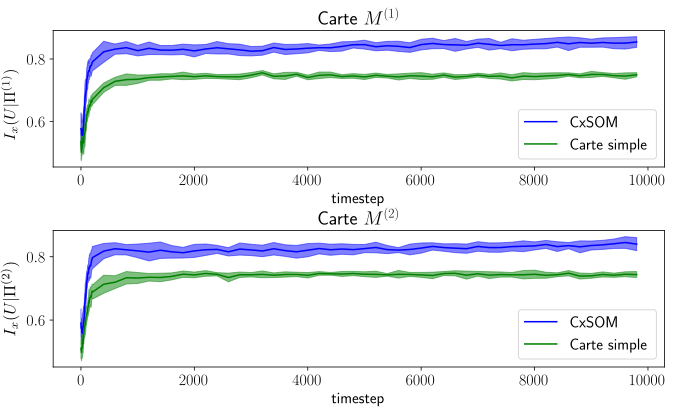
\includegraphics[width=0.8\textwidth]{evolution_MI_2}
\caption{\'Evolution de l'information mutuelle normalisée $I_x(U|\bmu)$ dans chaque carte au long de l'apprentissage.L'intervalle de discrétisation choisi pour $U$ est de $0.02$ (50 bins).
La courbe bleue correspond à $I_x(U|\bmu)$ dans l'architecture de cartes $M\m{1}$ et $M\m{2}$. On compare cette évolution à l'évolution de l'information d'une seule carte apprenant sur les mêmes entrées $\inpx\m{1}$ ou $\inpx\m{2}$, sans être connectée.}
\label{fig:MI_evol}
\end{figure}

\section{Comment utiliser l'information mutuelle continue comme indicateur d'un apprentissage ?}

Le ratio de corrélation et le coefficient d'incertitude, présentés ci-dessus, mesurent de deux manières différentes le fait que $U$ est une fonction du BMU dans chaque carte.
Bien que le coefficient d'incertitude s'appuie sur l'information mutuelle, l'indicateur que nous avons présenté se détache de la valeur théorique de l'information mutuelle par la discrétisation à gros grains de $U$.
Nous considérons qu'il restera intéressant d'étudier l'information mutuelle entre $U$ et les BMUs $\bmu\m{1}, \bmu\m{2}$ pour analyser l'apprentissage dans une architecture de cartes et présentons dans cette section des perspectives d'études de CxSOM par des mesures d'information mutuelle.

\subsection{\'Evolution de l'information mutuelle entre $U$ et $\bmu$ au cours d'un apprentissage}

En figure~\ref{fig:MI_evol_total}, nous traçons l'évolution de l'information mutuelle dans les deux cartes, estimée par la méthode de Kraskov. 
Nous observons que l'information mutuelle entre $U$ et $\bmu$ converge vers une valeur plus élevée dans une carte isolée que dans une architecture CxSOM.
Ce résultat est étonnant~: cela signifie donc que la carte au sein de CxSOM n'a pas plus d'information sur le modèle qu'une carte isolée. 
Ce résultat s'interprète par le fait que cette information n'est pas répartie de la même façon dans les deux expériences.
Dans une carte isolée, le niveau de quantification vectorielle sur $\inpx$ est très précis~: lorsqu'on présente une entrée $\inpx$ à la carte, le poids du BMU sera très proche de cette valeur $\inpx$. Or, la connaissance de $\inpx$ donne en soit beaucoup d'information sur le modèle $U$.
Dans CxSOM, on perd ce niveau de quantification sur $\inpx$, ce qu'on a observé en figure~\ref{fig:erreur}. On perd donc de l'information sur $\inpx$.

Le fait que l'information mutuelle soit plus élevée dans une carte indépendante dans les deux expériences traduit ainsi une perte d'information sur l'entrée $\inpx$ dans CxSOM par rapport à la carte indépendante, avec la perte de précision. Cette valeur ne traduit pas le gain d'information sur $\inpx\m{2}$ et donc $U$.
Les cartes effectuent donc un compromis~: chacune gagne de l'information sur le modèle $U$, au détriment de l'information apprise sur l'entrée externe. Ce comportement sera à valider sur d'autres modèles d'entrées.


Des méthodes permettant de séparer l'information entre variables existent dans la littérature. Elles nous permettraient de mesurer le gain d'information sur $U$ dans une ou plusieurs cartes sans s'intéresser à l'information apprise sur l'entrée externe $\inpx$.
Dans notre calcul du coefficient d'incertitude, c'est le fait de discrétiser grossièrement la distribution de $U$ qui a permis de mesurer le gain d'information sur $U$, sans prendre en compte le fait que la précision sur l'entrée externe est affaiblie.
Cette perte d'information pose néanmoins une question concernant la création d'architectures contenant plus de cartes~: jusqu'à quel point une carte peut-elle se permettre de perdre de l'information sur l'entrée externe pour gagner de l'information sur le modèle ? 
Cela motive l'idée qu'un apprentissage de $U$ dans une grande architecture devra être distribué entre les cartes et ne peut être appris indépendamment dans chaque carte.

\begin{figure}
\centering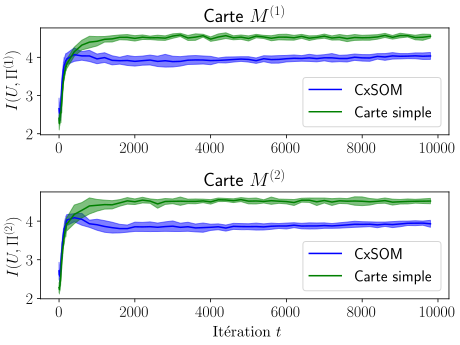
\includegraphics[width=0.8\textwidth]{evolution_MI_K_2}
\caption{\'Evolution de $I(U,\bmu)$ dans chaque carte au long de l'apprentissage, estimé par la méthode de Kraskov.
Cette valeur est moyennée sur 10 expériences. Nous comparons les valeurs obtenue dans une architecture CxSOM, en bleu, au cas d'une carte apprenant indépendamment sur les mêmes entrées $\inpx\m{1}$ et $\inpx\m{2}$.
Le même échantillon $U$ est utilisé pour chaque phase de test.
Nous pouvons voir que dans ces expériences, les positions des BMUs d'une carte indépendante partagent plus d'information avec $U$ que dans le cas de CxSOM. 
\label{fig:MI_evol_total}}
\end{figure}

\subsection{Ouvertures possibles}

Les mesures proposées dans ce chapitre ont permis d'évaluer un apprentissage du modèle indépendamment dans chaque carte.
La mesure de l'information mutuelle est cependant bien plus large que le seul calcul de $I(U,\bmu)$~; de nombreux aspects nous semblent intéressant à explorer pour une compréhension de l'apprentissage du modèle dans des architectures comportant plus de cartes. 
La méthode d'estimation par KNN présentée dans ce chapitre est une méthode classique d'estimation de l'information, mais il existe de nombreuses autres méthodes d'estimation \cite{Doquire2012ACO}. Des méthodes ont également été développées pour la mesure de l'information mutuelle entre variables continues et discrètes \cite{ross_mutual_2014, Gao2017EstimatingMI}. Enfin, l'information mutuelle a été utilisée pour analyser l'apprentissage dans des réseaux de neurones profonds en \cite{ShwartzZiv2017OpeningTB} ou encore directement comme métrique d'apprentissage en \cite{Hjelm2018LearningDR}.
Cette grandeur est donc bien documentée et donc pertinente à utiliser dans des travaux futurs.

Tout d'abord, il est possible de s'intéresser à la notion d'information mutuelle multivariée~: étant donné une variable cible $S$ et deux variables $R_1$ et $R_2$, $I(S;R_1,R_2)$ désigne l'information mutuelle entre $S$ et la variable jointe $(R_1,R_2)$. Nous pourrons ainsi mesurer, dans une architecture de cartes, $I(U; \bmu\m{1}, \bmu\m{2})$ par exemple.
Il est également possible de décomposer cette information multivariée~: \cite{williams_nonnegative_2010} définit, en plus de l'information mutuelle, la notion de redondance et de synergie entre variables, illustrée en figure \ref{fig:redondance}.
La redondance est l'information sur $S$ portée à la fois par $R_1$ et par $R_2$, et la synergie l'information portée seulement par la jointure des variables $R_1$ et $R_2$. Le calcul de telles grandeurs permettrait par exemple de séparer l'information gagnée sur $U$ et $\inpx$ dans une carte.
Le calcul de ces grandeurs entre les entrées, le modèle d'entrée et les BMUs des cartes CxSOM sont une piste d'étude pour une compréhension du stockage d'information dans une architecture de cartes et pour la définition d'un indicateur ciblant spécifiquement le gain d'information sur $U$.

\begin{figure}
    \centering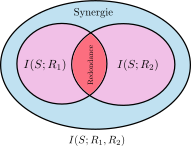
\includegraphics[width=0.5\textwidth]{redondance}
    \caption{Illustration des notions d'information \emph{redondante} et \emph{synergique} entre une variable $S$ et deux variables $R_1$ et $R_2$, schéma adapté de \cite{williams_nonnegative_2010}. \label{fig:redondance}
    }
\end{figure}
    

Des travaux comme \cite{lizier_detecting_2007,ceguerra_information_2011} s'intéressent quant à eux à la notion de transfert d'information au sein de systèmes dynamiques complexes. Le calcul d'information entre les éléments des cartes peut ainsi également s'appliquer à la quantification de la dynamique d'apprentissage d'une architecture de cartes.

La représentation des éléments d'une carte et des entrées d'un point de vue statistique que nous avons proposé dans cette thèse est ainsi une méthode pertinente pour la compréhension des comportements d'apprentissage du modèle CxSOM et leur analyse statistique reste à explorer dans des travaux futurs.
Nous avons en effet vu que les poids d'une carte et les mesures d'organisation seules ne traduisent pas forcément l'apprentissage des relations par les cartes de l'architecture. 
Cette approche "comportementale" rapproche les cartes de Kohonen d'autres algorithmes d'apprentissage non supervisés. Les perspectives d'études par l'information mutuelle mentionnées ci-dessus sont donc générales à tout type d'architecture d'apprentissage. Inversement, il sera possible d'appliquer des méthodes d'évaluation utilisées dans d'autres architectures afin de caractériser l'apprentissage associatif des cartes.


\section{Conclusion}

Ce chapitre utilise la méthode de représentation des éléments des cartes comme des variables aléatoires proposée au chapitre \ref{chap:repr} pour proposer des indicateurs de l'apprentissage multimodal au sein de l'architecture.
Les représentations visuelles sont en effet limitées dans des architectures de plus de deux ou trois cartes, et pour des données en plus grande dimension.

Dans ce chapitre, nous avons introduit deux indicateurs permettant de mesurer que $U$ est une fonction du $\bmu$ dans chacune des cartes de l'architecture. 
Nous avons en effet observé dans les deux chapitres précédents que ce comportement marque l'apprentissage du modèle dans des architectures de deux ou trois cartes en une dimension.

Nous avons introduit d'une part l'indicateur $I_x(U|\bmu)$ qui s'appuie sur l'information mutuelle entre $U$ et $\bmu$ et l'entropie de $U$. Cet indicateur a été étudié au début de la thèse.
L'indicateur $I_x$ que nous avons proposé correspond à une estimation d'une version normalisée de l'information mutuelle par la méthode des histogrammes, en discrétisant l'espace des variables $U$ et $\bmu$, avec une grande taille d'intervalle pour $U$. 
Ce découpage permet de ne pas prendre en compte le fait que les valeurs de $U$ encodées par une position de BMU $\bmu$ ont une dispersion locale, un bruit. Dans ce cas, l'indicateur permet d'évaluer numériquement si un BMU code pour un seul intervalle de valeur pour $U$ et non plusieurs comme dans le cas d'une carte simple. Il permet de comparer les expériences entre elles, donnant une valeur normalisée entre 0 et 1.
Il est cependant limité par la dimension de la variable $U$~: l'estimation par histogrammes, nécessite trop de points si $U$ dépasse la dimension 2 ou 3.

D'autre part, nous avons présenté le ratio de corrélation $\eta(U;\bmu)$, qui est une grandeur statistique mesurant directement la relation fonctionnelle entre $U$ et $\bmu$. Son calcul passe également par une discrétisation des positions $\bmu$, mais pas des valeurs de $U$. 
Dans un but de mesure de la relation fonctionnelle entre $U$ et $\bmu$, le ratio de corrélation sera donc à privilégier, car il est estimable pour des valeurs de $U$ en toute dimension et ne dépend pas de la taille d'intervalle choisie pour $U$.

La relation fonctionnelle entre $U$ et $\bmu$ n'est pas une propriété souhaitable dans des plus grandes architectures car elle suggère une perte d'information sur l'entrée externe au profit d'un grain d'information sur le modèle. On voudrait plutôt que la représentation de $U$ soit distribuée entre les cartes.
Pour étudier l'apprentissage multimodal dans un cadre plus général, nous suggérons aux travaux futurs de s'intéresser à l'information mutuelle et l'information multivariée entre $U$ et les valeurs des BMUs au sein des architectures de cartes.


\ifSubfilesClassLoaded{
    \printbibliography
    %\externaldocument{../main.tex}   
}{}
\end{document}

